% pandoc WBH Prüfungsvorlage
%
% Diese Vorlage ist für Prüfungen an der Wilhelm-Büchner-Hochschule erstellt worden
% sie entspricht den Vorgaben für Hausarbeiten und Thesis zum aktuellen Zeitpunkt.
% 
% Autoren:
%
% Created:
% Changed: 26.06.2020

\documentclass[
    12pt,
    a4paper,
            ngerman,
        bibliography=totocnumbered,
    listof=totocnumbered
]{scrartcl}

% Support different languages
% default: en
% -----------------------------------------------------------------------
\usepackage[shorthands=off,main=ngerman]{babel}


%\usepackage[utf8]{inputenc}
\usepackage[usenames,dvipsnames]{color}
\usepackage{amsmath}												% For pandoc extensive `amsmath` collection of symbols for typesetting ordinary math
\usepackage{amsfonts}												% More symboles for exotic currency notation and engeneering diagrams
\usepackage{amssymb}												% More symboles for exotic currency notation and engeneering diagrams
\usepackage{siunitx}                        % For using SI Units https://www.ctan.org/pkg/siunitx
\usepackage{fancyhdr}
\usepackage{tabularx}
\usepackage[a4paper, top=20mm, left=30mm, right=40mm, bottom=20mm, headsep=10mm, footskip=12mm]{geometry} % Vorgabe 4cm Rand auf der rechten Seite.
\usepackage{setspace}
\usepackage[right]{eurosym}
\usepackage[printonlyused]{acronym}
\usepackage{subfig}
\usepackage{floatflt}
\usepackage{colortbl}
\usepackage{paralist}
\usepackage{array}
\usepackage{parskip}
\usepackage[right]{eurosym}
\usepackage[subfigure,titles]{tocloft}
\usepackage{helvet}
\usepackage{graphicx}
\usepackage[export]{adjustbox} % also loads graphicx, to have max width for graphics
\usepackage{pdfpages}
\usepackage{tikz}


% ----------------------------------------------------------------------------------------------------------
% Firstname + Lastname
% ----------------------------------------------------------------------------------------------------------

% Firstname is set, assume name is Firstnaem + Lastname
\def \studentname{Sebastian Preisner}

% ----------------------------------------------------------------------------------------------------------
% Aufgabenstellung
% ----------------------------------------------------------------------------------------------------------
% Debug: 
% include:  file: Aufgabenstellung/Aufgabenstellung.pdf pages: 2-

\def \assignment{
    
% Regular include for historic reasons
%------------------
% include assignment is on
% \includepdf[pages=2-]{Aufgabenstellung/Aufgabenstellung.pdf}
% New include for historic reasons
%------------------

% check if assignment.file is set at all 
% check if form shall be filled out
\includepdf[pagecommand={  % 23mm, 6mm
\begin{tikzpicture}[remember picture, overlay, x=1mm,y=1mm,%
mybox/.style={rectangle,minimum width=56mm, draw opacity=0.0, line width=0,  minimum height=8mm, align=left,text width=56mm},%
info/.style={mybox,draw=black,align=left}]
\node at (34,-34) [info] {Sebastian};
\node at (95,-34) [info] {Preisner};
\node at (34,-47) [info] {Hilpertstr. 31};
\node at (95,-47) [info] {64295 Darmstadt}; 
\node at (34,-59) [info] {900266};
\node at (95,-59) [info] {1140};
\end{tikzpicture}}, pages=1]{Aufgabenstellung/Aufgabenstellung.pdf}
 % check if we need to include the rest of the document
\includepdf[pages=2-]{Aufgabenstellung/Aufgabenstellung.pdf} % Include rest of document

}



\usepackage{multirow}


% Support hyperref with colorisation
% -------------------------------------------------------------------------
\usepackage{xcolor}
\IfFileExists{xurl.sty}{\usepackage{xurl}}{} % add URL line breaks if available
\IfFileExists{bookmark.sty}{\usepackage{bookmark}}{\usepackage[pdfpagelabels=true]{hyperref}}
\urlstyle{same} % disable monospaced font for URLs




\setlength{\emergencystretch}{3em} % prevent overfull lines

% PDF Metadata
% ------------------------------------------------------------------
\hypersetup{
	unicode=false, 
	pdftoolbar=true, 
	pdfmenubar=true, 
	pdffitwindow=false, 
	pdfstartview={FitH},
	pdftitle={Pandoc und Markdown für deine
Texte: Freiwillige\_Arbeit- \studentname},
	pdfauthor={Sebastian Preisner, Matrikelnummer: 900266},
		pdfsubject={Studiengang: Technische Informatik}, 
		pdfcreator={\LaTeX\ with package \flqq hyperref\frqq via pandoc},
	pdfproducer={pdfTeX \the\pdftexversion.\pdftexrevision},
	pdfkeywords={B-Prüfung, 900266, Freiwillige\_Arbeit, },
	pdfnewwindow=true,
		pdflang=de,
		pdfdisplaydoctitle=true, 
		hidelinks,
	}

% Designing blockquote
% ------------------------------------------------------------------
\definecolor{blockquote-border}{RGB}{221,221,221}
\definecolor{blockquote-text}{RGB}{119,119,119}
\usepackage{mdframed}
\newmdenv[rightline=false,bottomline=false,topline=false,linewidth=3pt,linecolor=blockquote-border,skipabove=\parskip]{customblockquote}
\renewenvironment{quote}{\begin{customblockquote}\list{}{\rightmargin=0em\leftmargin=0em}%
\item\relax\color{blockquote-text}\ignorespaces}{\unskip\unskip\endlist\end{customblockquote}}

% Syntax Highlighting with colors
% -----------------------------------------------------------------
\usepackage{color}
\usepackage{fancyvrb}
\newcommand{\VerbBar}{|}
\newcommand{\VERB}{\Verb[commandchars=\\\{\}]}
\DefineVerbatimEnvironment{Highlighting}{Verbatim}{commandchars=\\\{\}}
% Add ',fontsize=\small' for more characters per line
\newenvironment{Shaded}{}{}
\newcommand{\AlertTok}[1]{\textcolor[rgb]{1.00,0.00,0.00}{\textbf{#1}}}
\newcommand{\AnnotationTok}[1]{\textcolor[rgb]{0.38,0.63,0.69}{\textbf{\textit{#1}}}}
\newcommand{\AttributeTok}[1]{\textcolor[rgb]{0.49,0.56,0.16}{#1}}
\newcommand{\BaseNTok}[1]{\textcolor[rgb]{0.25,0.63,0.44}{#1}}
\newcommand{\BuiltInTok}[1]{#1}
\newcommand{\CharTok}[1]{\textcolor[rgb]{0.25,0.44,0.63}{#1}}
\newcommand{\CommentTok}[1]{\textcolor[rgb]{0.38,0.63,0.69}{\textit{#1}}}
\newcommand{\CommentVarTok}[1]{\textcolor[rgb]{0.38,0.63,0.69}{\textbf{\textit{#1}}}}
\newcommand{\ConstantTok}[1]{\textcolor[rgb]{0.53,0.00,0.00}{#1}}
\newcommand{\ControlFlowTok}[1]{\textcolor[rgb]{0.00,0.44,0.13}{\textbf{#1}}}
\newcommand{\DataTypeTok}[1]{\textcolor[rgb]{0.56,0.13,0.00}{#1}}
\newcommand{\DecValTok}[1]{\textcolor[rgb]{0.25,0.63,0.44}{#1}}
\newcommand{\DocumentationTok}[1]{\textcolor[rgb]{0.73,0.13,0.13}{\textit{#1}}}
\newcommand{\ErrorTok}[1]{\textcolor[rgb]{1.00,0.00,0.00}{\textbf{#1}}}
\newcommand{\ExtensionTok}[1]{#1}
\newcommand{\FloatTok}[1]{\textcolor[rgb]{0.25,0.63,0.44}{#1}}
\newcommand{\FunctionTok}[1]{\textcolor[rgb]{0.02,0.16,0.49}{#1}}
\newcommand{\ImportTok}[1]{#1}
\newcommand{\InformationTok}[1]{\textcolor[rgb]{0.38,0.63,0.69}{\textbf{\textit{#1}}}}
\newcommand{\KeywordTok}[1]{\textcolor[rgb]{0.00,0.44,0.13}{\textbf{#1}}}
\newcommand{\NormalTok}[1]{#1}
\newcommand{\OperatorTok}[1]{\textcolor[rgb]{0.40,0.40,0.40}{#1}}
\newcommand{\OtherTok}[1]{\textcolor[rgb]{0.00,0.44,0.13}{#1}}
\newcommand{\PreprocessorTok}[1]{\textcolor[rgb]{0.74,0.48,0.00}{#1}}
\newcommand{\RegionMarkerTok}[1]{#1}
\newcommand{\SpecialCharTok}[1]{\textcolor[rgb]{0.25,0.44,0.63}{#1}}
\newcommand{\SpecialStringTok}[1]{\textcolor[rgb]{0.73,0.40,0.53}{#1}}
\newcommand{\StringTok}[1]{\textcolor[rgb]{0.25,0.44,0.63}{#1}}
\newcommand{\VariableTok}[1]{\textcolor[rgb]{0.10,0.09,0.49}{#1}}
\newcommand{\VerbatimStringTok}[1]{\textcolor[rgb]{0.25,0.44,0.63}{#1}}
\newcommand{\WarningTok}[1]{\textcolor[rgb]{0.38,0.63,0.69}{\textbf{\textit{#1}}}}


\renewcommand{\familydefault}{\sfdefault}

% Pandoc tightlisting
% ------------------------------------------------------------------
\providecommand{\tightlist}{%
  \setlength{\itemsep}{0pt}\setlength{\parskip}{0pt}}


% Support for citation
% -------------------------------------------------------------------

\usepackage[T1]{fontenc}


%
	\setcounter{secnumdepth}{5}
	%\setcounter{secnumdepth}{-\maxdimen} % remove section numbering

% ----------------------------------------------------------------------------
% begin document
% ----------------------------------------------------------------------------

\begin{document}


%
% Assignment
% -------------------
\assignment

% ----------------------------------------------------------------------------------------------------------
% Kopf und Fußzeile
% ----------------------------------------------------------------------------------------------------------
\renewcommand{\sectionmark}[1]{\markright{#1}}
\renewcommand{\leftmark}{\rightmark}
\pagestyle{fancy}
\lhead{}
\chead{}
\rhead{\thesection\space\contentsname}
\lfoot{\tiny B-Prüfung des Studenten: Sebastian
Preisner (Matrikelnr.: 900266) Studiengang: Technische
Informatik - Prüfung: Freiwillige\_Arbeit }
\cfoot{}
\rfoot{\ \linebreak Seite \thepage}
\renewcommand{\headrulewidth}{0.4pt}
\renewcommand{\footrulewidth}{0.4pt}

% Vorspann
\renewcommand{\thesection}{\Roman{section}}
\renewcommand{\theHsection}{\Roman{section}}
\pagenumbering{Roman}

% Pagebreak after each Section
\let\oldsection\section
\renewcommand\section{\clearpage\oldsection}

% ----------------------------------------------------------------------------------------------------------
% Titelseite
% ----------------------------------------------------------------------------------------------------------
\thispagestyle{empty}
\begin{center}
    \includegraphics[max width=\textwidth]{../Bilder/logo.png}\\    
    \vspace*{2cm}
	\Large
			\textbf{Studiengang:}\\
		\textbf{Technische Informatik}\\
		\vspace*{1cm}
		\Huge
			\textbf{}\\
		\vspace*{0.5cm}
				\textbf{Pandoc und Markdown für deine Texte} \\
		\vspace*{0.3cm}
	\large
  		Freiwillige\_Arbeit \\
		\vspace*{0.5cm}
			\textbf{Freizeitgestaltung}\\
		\vspace*{0.5cm}
	
	\vfill
	\normalsize
	\newcolumntype{x}[1]{>{\raggedleft\arraybackslash\hspace{0pt}}p{#1}}
	\begin{tabular}{x{6cm}p{7.5cm}}
					\rule{0mm}{5ex}\textbf{Student:} & \studentname
							\newline Hilpertstr. 31
										\newline 64295 Darmstadt
										\newline wbh@calyrium.org
			 \\
									\rule{0mm}{5ex}\textbf{Matrikelnummer:} & 900266 \\
							\rule{0mm}{5ex}\textbf{Abgabedatum:} & 08.06.2017 \\
			\end{tabular}
\end{center}
\pagebreak

% ----------------------------------------------------------------------------------------------------------
% Assignment
% ----------------------------------------------------------------------------------------------------------



 % Skip first page count, if skipfirstpage = 1
\clearpage
\setcounter{page}{1}





{

\setcounter{tocdepth}{3}

% ----------------------------------------------------------------------------------------------------------
% Inhaltsverzeichnis
% ----------------------------------------------------------------------------------------------------------
% TODO Typ vor Nummer
\renewcommand{\cfttabpresnum}{Tab. }
\renewcommand{\cftfigpresnum}{Abb. }
\settowidth{\cfttabnumwidth}{Abb. 10\quad}
\settowidth{\cftfignumwidth}{Abb. 10\quad}

\singlespacing
\rhead{INHALTSVERZEICHNIS}
\renewcommand{\contentsname}{I Inhaltsverzeichnis}
\phantomsection
\addcontentsline{toc}{section}{\texorpdfstring{I \hspace{0.35em}Inhaltsverzeichnis}{Inhaltsverzeichnis}}
\addtocounter{section}{1}
\tableofcontents
\pagebreak
}




% ----------------------------------------------------------------------------------------------------------
% Einrichtung der Kopfzeile
% ----------------------------------------------------------------------------------------------------------
\renewcommand{\sectionmark}[1]{\markright{#1}}
\renewcommand{\subsectionmark}[1]{}
\renewcommand{\subsubsectionmark}[1]{}
\lhead{Abschnitt \thesection}
\rhead{} %hier kann die rechte Seite der Kopfzeile editiert werden!

\onehalfspacing
\renewcommand{\thesection}{\arabic{section}}
\renewcommand{\theHsection}{\arabic{section}}
\setcounter{section}{0}
\pagenumbering{arabic}
\setcounter{page}{1}
%\renewcommand{\includegraphics}[1][]{\includegraphics[width=0.9\columnwidth,keepaspectratio]{#1}}


% ----------------------------------------------------------------------------------------------------------
% Inhalt
% ----------------------------------------------------------------------------------------------------------

\hypertarget{einfuxfchrungauthor}{%
\section{Einführungauthor}\label{einfuxfchrungauthor}}

Im Folgenden möchte ich dir Pandoc und Markdown näher bringen und dir
zeigen wieso du in Zukunft nur noch so schreiben möchtest. Dabei werde
ich zunächst ein grobes Bild von Pandoc und Markdown zeichnen und dir im
weiteren Verlauf die Installation und den Einsatz näher bringen und zum
Schluss gehe ich nochmal speziell auf diese Vorlage für Pandoc ein.

\hypertarget{was-ist-markdown}{%
\subsection{Was ist Markdown?}\label{was-ist-markdown}}

Markdown ist eine Auszeichnungssprache und wurde maßgeblich von den
frühen Text-E-Mails beeinflusst. Zu Zeiten wo man noch keine E-Mails mit
Überschriften, kursiver und fettgedruckter Schrift usw. verfassen konnte
musste man sich anderweitig behelfen. Das Ziel von Markdown ist die
Lesbarkeit und einfache Schreibbarkeit von Texten. Das ermöglicht dem
Schreiber eine hohe Konzentration auf den Text und wenig ablenkung durch
Formatierungen verglichen WISIWYG (What you see is what you get)
Editoren wie Microsoft Word. Zur Veranschaulischung möchte ich dir hier
kruz ein paar Formatierungen im Dokument zeigen:

Blockquote:

\begin{quote}
Lorem ipsum dolor sit amet, consectetur adipisicing elit, sed do eiusmod
tempor incididunt ut labore et dolore magna aliqua. Ut enim ad minim
veniam, quis nostrud exercitation ullamco laboris nisi ut aliquip ex ea
commodo consequat. Duis aute irure dolor in reprehenderit in voluptate
velit esse cillum dolore eu fugiat nulla pariatur. Excepteur sint
occaecat cupidatat non proident, sunt in culpa qui officia deserunt
mollit anim id est laborum.
\end{quote}

Codeblock:

\begin{Shaded}
\begin{Highlighting}[]
\FunctionTok{\# Überschrift 1. Grades}
\FunctionTok{\#\# Überschrift 2. Grades}

\SpecialStringTok{* }\NormalTok{Listenpunkt 1}
\SpecialStringTok{* }\NormalTok{Listenpunkt 2}
\SpecialStringTok{* }\NormalTok{Listenpunkt 3}

\NormalTok{Ich bin ein Text mit *kursiven* und **fetten** Elementen.}
\end{Highlighting}
\end{Shaded}

Anhand dieses Beispiels kann man sehen wie einfach das Schreiben von
Markdown ist. Nun wirst du dir sicherlich denken was dir diese
einfachheit bringt wenn dein Dokument aber aussieht wie E-Mails vor 10
Jahren. Die Antwort darauf ist, das sich in den ganzen Jahren viele
Parser für Markdown entwickelt haben welche die einfache Syntax nutzen
um perfekt Formatierte Texte zu erstellen. Eines dieser Tools und noch
dazu das wohl mächtigste, ist Pandoc.

\hypertarget{was-ist-pandoc}{%
\subsection{Was ist Pandoc?}\label{was-ist-pandoc}}

\href{http://pandoc.org/}{Pandoc} ist ein Übersetzer der eine Datei von
einem Markup in ein anderes übersetzt. Markup ist das englische Wort für
Auszeichnung und steht für eine maschinenlesbare Sprache für die
Gliederung und Formatierung von Texten und Daten. Der bekannteste
Vertreter ist sicherlich die Hypertext Markup Language (HTML), die
Kernsprache des World Wide Webs. Pandoc bassiert hierbei auf einer
erweiterten Variante der Auszeichnungssprache Markdown.

Im folgenden findest du einige input Formate die von Pandoc unterstützt
werden. Eine volle liste findest du auf der Webseite von
\href{http://pandoc.org/}{Pandoc}.

\begin{itemize}
\tightlist
\item
  Markdown
\item
  CommonMark
\item
  LaTeX
\item
  textil
\item
  HTML
\item
  EPUB
\item
  LibreOffice/OpenOffice (odt)
\item
  Microsoft Word DOCX (OOXML)
\item
  Mediawiki
\item
  DocBook
\end{itemize}

Alle diese Formate unterstützt Pandoc auch für den Export und
zusätzlich:

\begin{itemize}
\tightlist
\item
  PDF via LaTeX
\item
  Dokumentationsformate: DocBook, GNU TexInfo, Groff manpages
\item
  HTML5, XHTML
\item
  AsciiDoc
\end{itemize}

\hypertarget{wieso-sollte-ich-pandoc-einsetzen}{%
\subsection{Wieso sollte ich Pandoc
einsetzen?}\label{wieso-sollte-ich-pandoc-einsetzen}}

Hierfür gibt es viele gute Argumente. Zum einen kannst du deine
geschriebene Arbeit

\hypertarget{installation-und-einrichtung}{%
\section{Installation und
Einrichtung}\label{installation-und-einrichtung}}

In diesem Kapitel geht es um die Installation und die Einrichtung der
Tools. Da ich persönlich kein Windows besitze richtet sich die Anleitung
ausschließlich an Linux nutzer. Ich würde mich jedoch über ergänzende
Beiträge freuen.

\hypertarget{markdown}{%
\subsection{Markdown}\label{markdown}}

Da Markdown lediglich eine Auszeichnungssprache ist benötigst du
eigentlich nichts außer einen Texteditor. Diesen findet man unter allen
gängigen Betriebssystemen. Auch auf der Konsole oder in diversen
Webeditoren lässt sich Markdown schreiben (z.B. in einer E-Mail bei
einem Mailprovider). Du merkst, durch die Einfachheit ist dir bei der
Bearbeiten von Texten absolut keine grenze gesetzt und du wirst keine
Probleme haben das Dokument auf irgend einem deiner Endgeräte (z.B.
Computer, Laptop, Smartphone) zu öffnen und zu bearbeiten. Selbst auf
der Arbeit sollte es für dich möglich sein (sofern du die Datei auf den
Computer drauf und auch wieder herrunter bekommst, kläre dies bitte
vorher mit deinem Arbeitgeber) deine Arbeiten zu vervollständigen.

Als Hilfe gibt es jedoch eine lange Liste an Markdown Editoren die dir,
meist in einem Splitscreen, das Ergebnis direkt anzeigen. Den größten
mir bekannten Umfang bietet ganz klar Atom, dabei handelt es sich nicht
um einen reinen Markdown Editor sondern um eine Texteditor der mit
vielen zusätzlichen Plugins erweitert werden kann. Er ist OpenSource und
steht für alle Plattformen zur verfügung.

\hypertarget{pandoc}{%
\subsection{Pandoc}\label{pandoc}}

Pandoc findest du in den gängigen Linux Distributionen in deren
Repositories. Den Befehl zur Installtion für einige Distributionen
findest du in der folgenden Box. Um Dateien in ein PDF Übersetzen zu
können benötigt Pandoc noch LaTeX. Die LaTeX Umgebung ist sehr groß, wer
also auf Speicherplatz achten muss, dem empfehle ich sich mit den
benötigten Packeten auseinander zu setzen. Ansonsten ist eine volle
Installation von LaTeX der einfachste Weg.

\begin{Shaded}
\begin{Highlighting}[]
\CommentTok{\# Ubuntu, Kubuntu, Mint}
\FunctionTok{sudo}\NormalTok{ apt{-}get install pandoc}

\CommentTok{\# Fedora}
\ExtensionTok{yum}\NormalTok{ install pandoc}

\CommentTok{\# Archlinux}
\ExtensionTok{pacman} \AttributeTok{{-}S}\NormalTok{ pandoc}
\end{Highlighting}
\end{Shaded}

Eine grafische Oberfläche wirst du bei Pandoc nicht finden, das Programm
wird mit Hilfe von Befehlen auf der Konsole bedient. Da es sich um einen
Übersetzer handelt ist dies aber kein Problem denn alle Einstellungen
lassen sich Bequem in Textfom fomulieren. Wie das geht werde ich dir im
nächsten Kapitel zeigen. Zunächst kannst du jedoch mit dem Befehl
\texttt{pandoc\ -v} die installierte Version erfragen.

\hypertarget{pdf-aus-beispiel-markdown-erzeugen}{%
\subsection{PDF aus Beispiel Markdown
erzeugen}\label{pdf-aus-beispiel-markdown-erzeugen}}

\hypertarget{manuell}{%
\subsubsection{Manuell}\label{manuell}}

Dem Projekt liegt im Ordner \texttt{Beispiel/} ein in Markdown
geschriebenes Beispiel bei, welches du gerade liest :-)

Du kannst das Beispiel mit Markdown nach PDF konvertieren in dem du
folgendes Kommando nutzt:

\texttt{pandoc\ -s\ -\/-template="wbh.tex"\ -o\ Beispiel/beispiel.pdf\ Beispiel/beispiel.md}

Die Datei \texttt{beispiel.pdf} wird ebenfalls im Unterordner
\texttt{Beispiel/}erzeugt. Das Kommando musst du natürlich aus dem
Stammverzeichnis des Projekts starten, damit das Template
\texttt{wbh.tex} gefunden wird. Alternativ kannst du auch den Pfad
anpassen.

\hypertarget{uxfcber-editor}{%
\subsubsection{Über Editor}\label{uxfcber-editor}}

Viele Editoren erlauben, dass du Quellcode über ein Tastaturkürzel, z.b.
F5 oder F9 automatisch kompilieren kannst. Bei der Vielzahl der Editoren
ist es schwierig das für alle zu beschreiben, es lohnt sich trotzdem in
den Einstellungen zu prüfen ob das mit deinem Editor möglich ist. Jeder
bessere Sourcecode Editor kann das.

\hypertarget{latex-mathtex-beispiele}{%
\section{Latex Mathtex Beispiele}\label{latex-mathtex-beispiele}}

Hier ein paar Beispiele für mathematische Formeln

\hypertarget{matrix}{%
\subsection{Matrix}\label{matrix}}

Wenn die Matrix mehr als 10 Spalten enthält, dann muss zwingend
\texttt{\textbackslash{}setcounter\{MaxMatrixCols\}\{12\}} entsprechend
der Anzahl der Spalten gesetzt sein. Standarmäßig geht es sonst nur bis
10 Spalten.

\[
\setcounter{MaxMatrixCols}{12}X = 
 \begin{pmatrix}
P(A) & P(B) & P(C) & P(D) & P(E) & P(F) & P(G) & P(H) & P(I) & P(J) & P(K) & P(L)\\
1/19 & 2/19 & 3/19 & 3/19 & 3/19 & 1/19 & 1/19 & 1/19 & 1/19 & 1/19 & 1/19 & 1/19\\
\end{pmatrix}\]

\hypertarget{am-gleichheitszeichen-ausgerichtete-gleichungen}{%
\subsection{Am Gleichheitszeichen ausgerichtete
Gleichungen}\label{am-gleichheitszeichen-ausgerichtete-gleichungen}}

Wenn du Gleichungen über mehrere Zeilen schreist und diese am
Gleichheitszeichen ausrichten möchtest, dann nutze
\texttt{\textbackslash{}begin\{aligned\}}. Zeilenumbrüche fügst du mit
\texttt{\textbackslash{}\textbackslash{}} hinzu.

Die Ausrichtung richtet sich am \texttt{\&} welches als Spaltenseparator
dient.

\[ \displaystyle
\begin{aligned}
A &  = B + C + D + E + F\\
& \\
 A - F & = B + C + D + E 
\end{aligned}\]

% ----------------------------------------------------------------------------------------------------------
% Literaturverzeichnis
% ----------------------------------------------------------------------------------------------------------




%%%

%

\end{document}
